\documentclass[12pt]{article}
\usepackage[utf8]{inputenc}
\usepackage[a4paper, margin=2cm]{geometry}
\usepackage{amsthm}
\usepackage{amsmath, amssymb}
\usepackage{circuitikz}
\usepackage{graphicx}
\usepackage{karnaugh-map}
\usepackage{newtxtext, newtxmath}
\usepackage{pgfplots}
\usepackage{tcolorbox}
\usepackage{tikz}
\usepackage{titlesec}
\usepackage{xcolor}
\usepackage{listings}
\usepackage{xeCJK}
\usetikzlibrary{patterns,arrows,decorations.pathmorphing}
\definecolor{lightblue}{RGB}{135, 206, 250}
\definecolor{commentgreen}{rgb}{0.25,0.5,0.35}
\definecolor{keywordblue}{rgb}{0.13,0.13,1}
\definecolor{stringmagenta}{rgb}{0.5,0,0.35}
\tcbuselibrary{skins,theorems}

\titleformat{\section}[block]{\Large\bfseries\centering}{}{0pt}{}
\titleformat{\subsection}[block]{\bfseries}{\thesubsection}{2pt}{}

\lstdefinestyle{verilogstyle}{
  language=Verilog,                % 设置语言
  backgroundcolor=\color{white},   % 背景色
  commentstyle=\color{commentgreen},% 注释样式
  keywordstyle=\color{keywordblue}, % 关键字样式
  numberstyle=\tiny\color{gray},    % 行号的样式
  stringstyle=\color{stringmagenta},% 字符串样式
  basicstyle=\ttfamily\small,      % 代码基本样式
  breakatwhitespace=false,         % 是否只在空白处换行
  breaklines=true,                 % 自动换行
  captionpos=b,                    % 标题位置（底部）
  keepspaces=true,                 % 保留空格
  numbers=left,                    % 行号的位置
  numbersep=5pt,                   % 行号与代码的距离
  showspaces=false,                % 是否显示空格
  showstringspaces=false,          % 字符串中的空格是否显示
  showtabs=false,                  % 是否显示制表符
  tabsize=2,                       % 制表符的宽度
  frame=single,                    % 边框样式
  rulecolor=\color{black}          % 边框颜色
}

% 创建一个新的listings环境
\lstnewenvironment{verilogcode}[1][]
{
  \lstset{style=verilogstyle, #1} % 使用Verilog样式，允许自定义设置
}{}

\newtcbtheorem[no counter]{proposition}{\large\hspace{-8pt}Proposition}{
  enhanced,
  colback=white,
  colframe=lightblue,
  left=12pt,
  right=12pt,
  top=24pt,
  bottom=24pt,
  fonttitle=\bfseries
}{prop}
\newtcbtheorem[]{question}{\large\hspace{-8pt}Question :}{
  enhanced,
  colback=white,
  colframe=black,
  left=12pt,
  right=12pt,
  top=24pt,
  bottom=24pt,
  fonttitle=\bfseries
}{qst}
\newenvironment{Answer}{
  \vspace{12pt}
  {\large\textbf{\textit{\hspace{-12pt}Answer:}}}\par
  \vspace{8pt}
} {\vspace{24pt}}
\newenvironment{Proof}{
  \vspace{12pt}
  {\large\textbf{\textit{\hspace{-12pt}Proof:}}}\par
  \vspace{8pt}
} {\vspace{24pt}}

\title{DCHw1}
\author{Miki-Riako }
\date{\today}
\begin{document}

\begin{question}{}{}
  5-2 Draw the waveform of Q.
\end{question}
\begin{Answer}
由于SR锁存器的特征方程：
$$Q^{n+1}=S+\overline RQ^n$$
$$SR=0$$

可知图形如下：

\begin{center}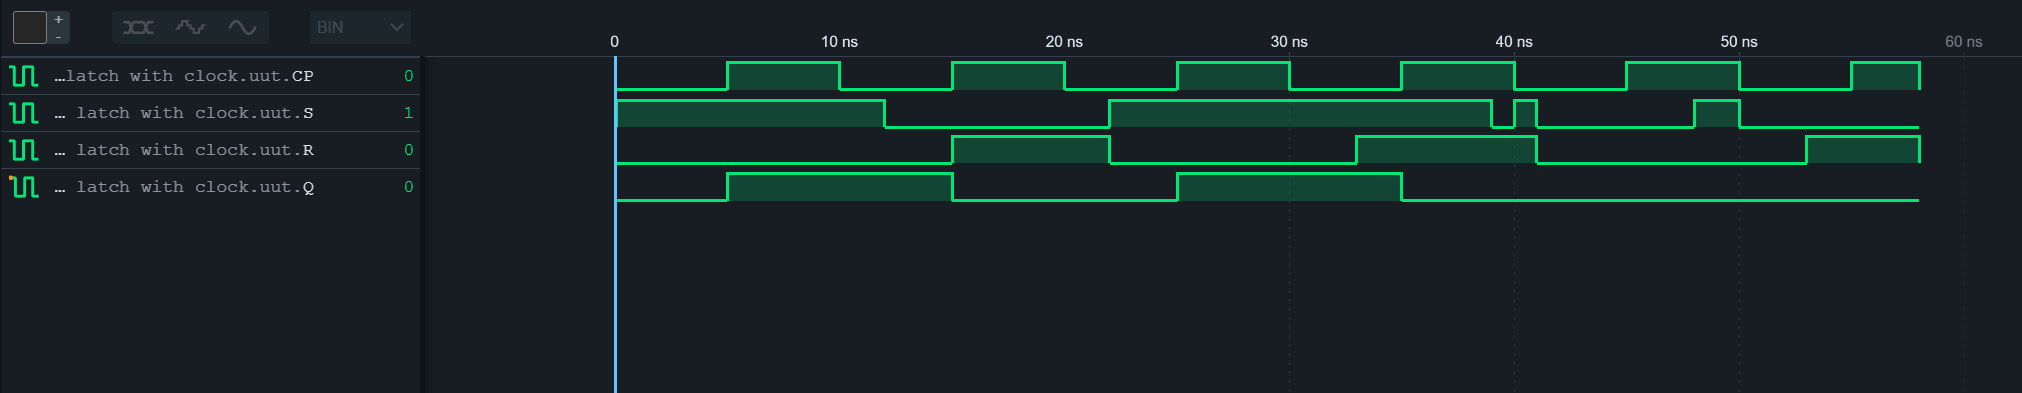
\includegraphics[width=1\textwidth]{image/wave_1.png}\end{center}

经过验证后输出正确。
\end{Answer}

\begin{question}{}{}
  5-3 Analyze the functions and the equation.
\end{question}
\begin{Answer}
(a)
由于SR锁存器的特征方程：
$$Q^{n+1}=S+\overline RQ^n$$
$$SR=0$$

代入$S=A\overline Q$与$R=BQ$，得到：

$$Q^{n+1}=A\overline {Q^n}+\overline {BQ^n}Q^n$$
$$SR=0$$

化简即为：

$$Q^{n+1}=A\overline {Q^n}+\overline BQ^n$$
$$SR=0$$

(b)
同理，由$S=C\overline Q$与$R=D\overline Q$，得到：

$$Q^{n+1}=C\overline {Q^n}+\overline {D\overline{Q^n}}Q^n$$
$$SR=0$$

化简即为：

$$Q^{n+1}=C+Q^n$$
$$SR=0$$

\end{Answer}

\begin{question}{}{}
  5-9 Draw the waveform of Q and Z.
\end{question}
\begin{Answer}
由D触发器的公式$Q^{n+1}=D$得到如图所示：

\begin{center}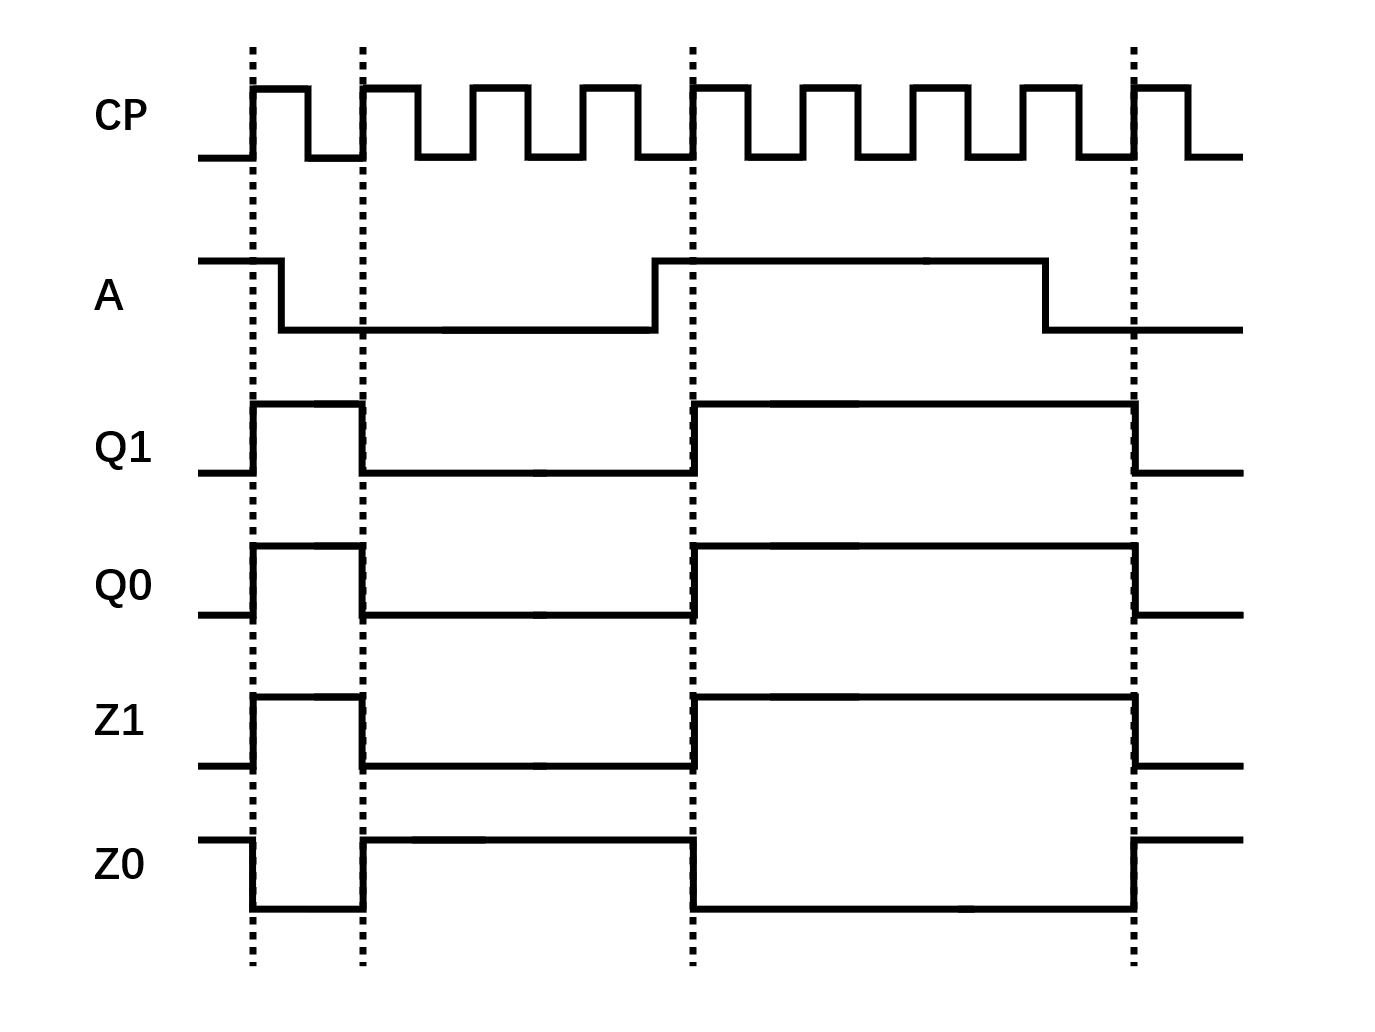
\includegraphics[width=0.6\textwidth]{image/wave_2.png}\end{center}
\end{Answer}

\begin{question}{}{}
  5-10 Draw the waveform of Q and Z.
\end{question}
\begin{Answer}
由JK触发器的公式$Q^{n+1}=J\overline {Q^n}+\overline KQ^n$，化简得到：

$$Q_0^{n+1}=\overline {Q_0^n}+Q_0^n=1$$
$$Q_1^{n+1}=\overline {Q_1^n}+Q_1^n=1$$
$$Z=\overline{Q_0^{n+1}\overline{Q_1^{n+1}}}=\overline{Q_0^{n+1}}+Q_1^{n+1}$$

得到如图所示：

\begin{center}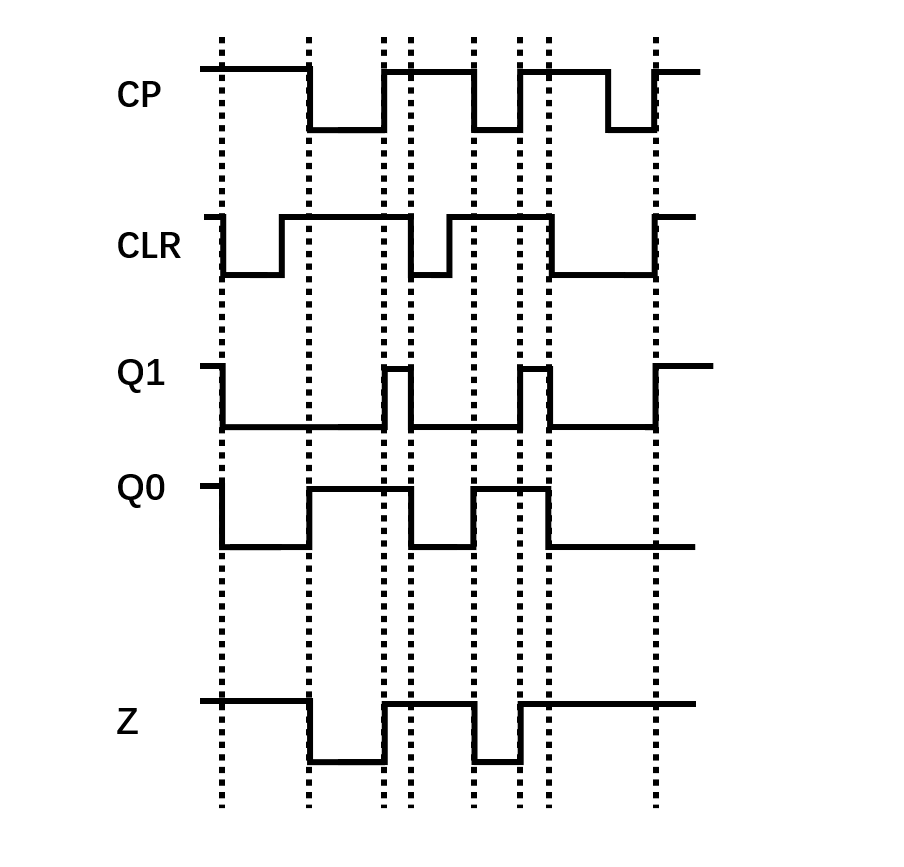
\includegraphics[width=0.6\textwidth]{image/wave_3.png}\end{center}
\end{Answer}

\begin{question}{}{}
  5-13 Draw the waveform of Q.
\end{question}
\begin{Answer}
由JK触发器的公式$Q^{n+1}=J\overline {Q^n}+\overline KQ^n$得到如图所示：

\begin{center}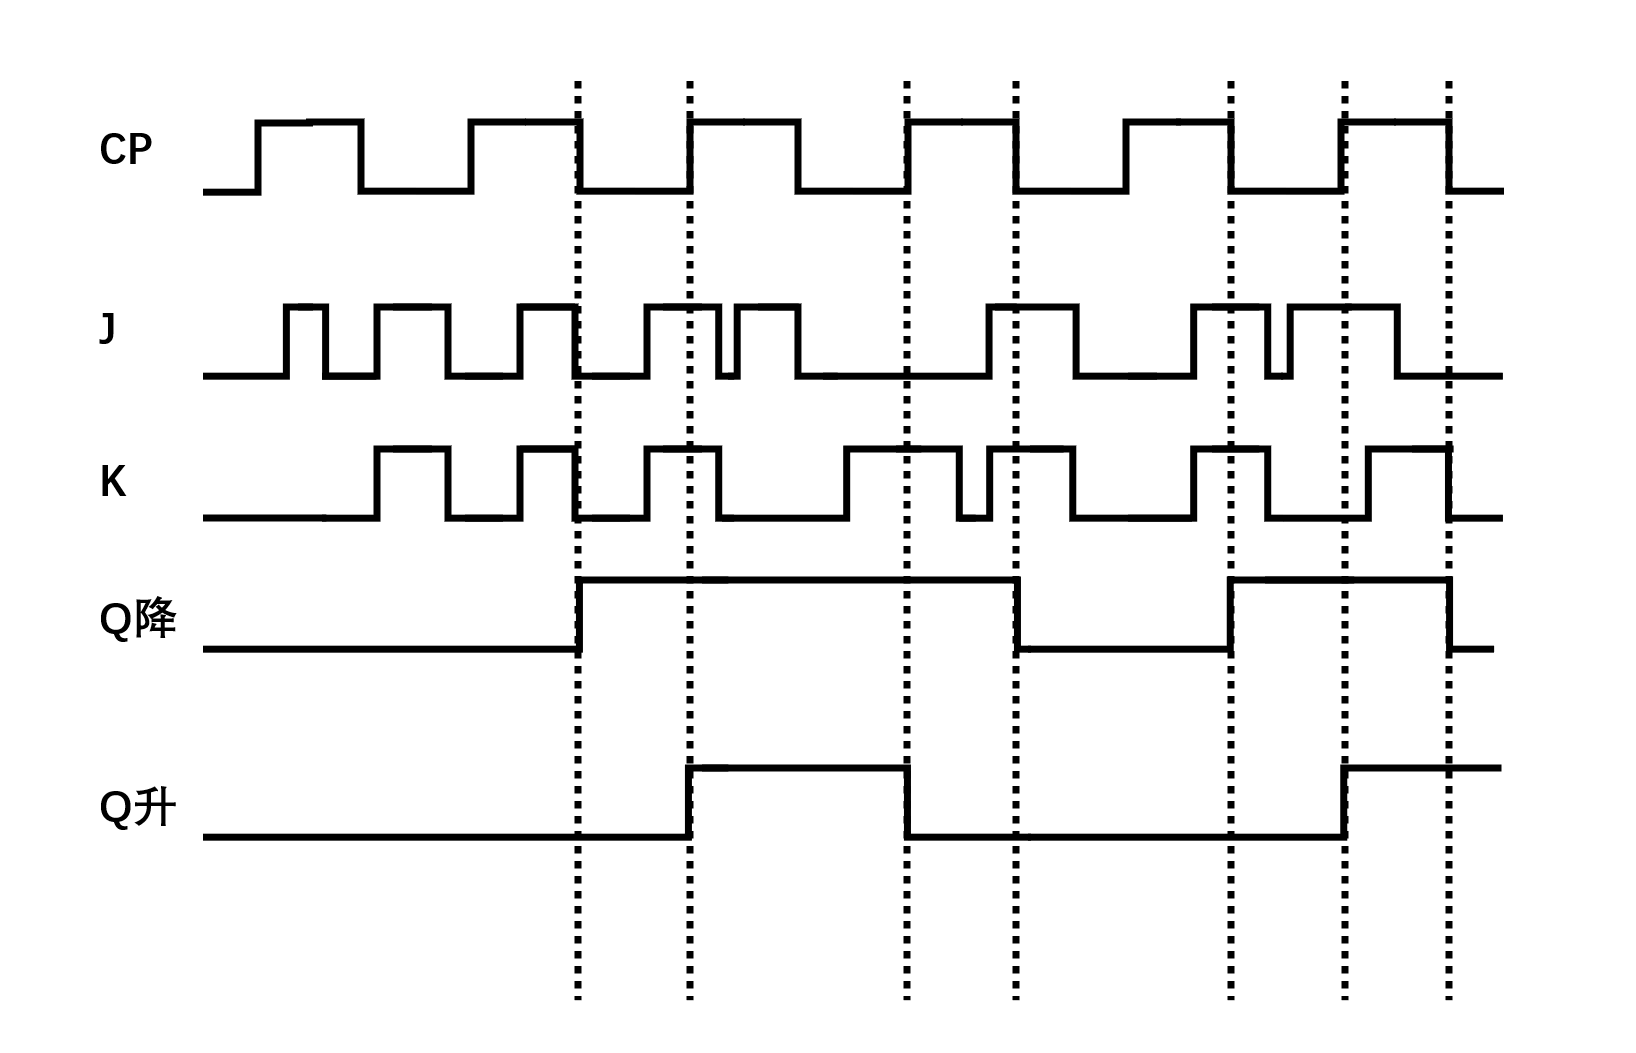
\includegraphics[width=0.6\textwidth]{image/wave_4.png}\end{center}
\end{Answer}

\begin{question}{}{}
  5-14 Draw the waveform of Q.
\end{question}
\begin{Answer}
同理，根据题目所述，绘制图如下：
\begin{center}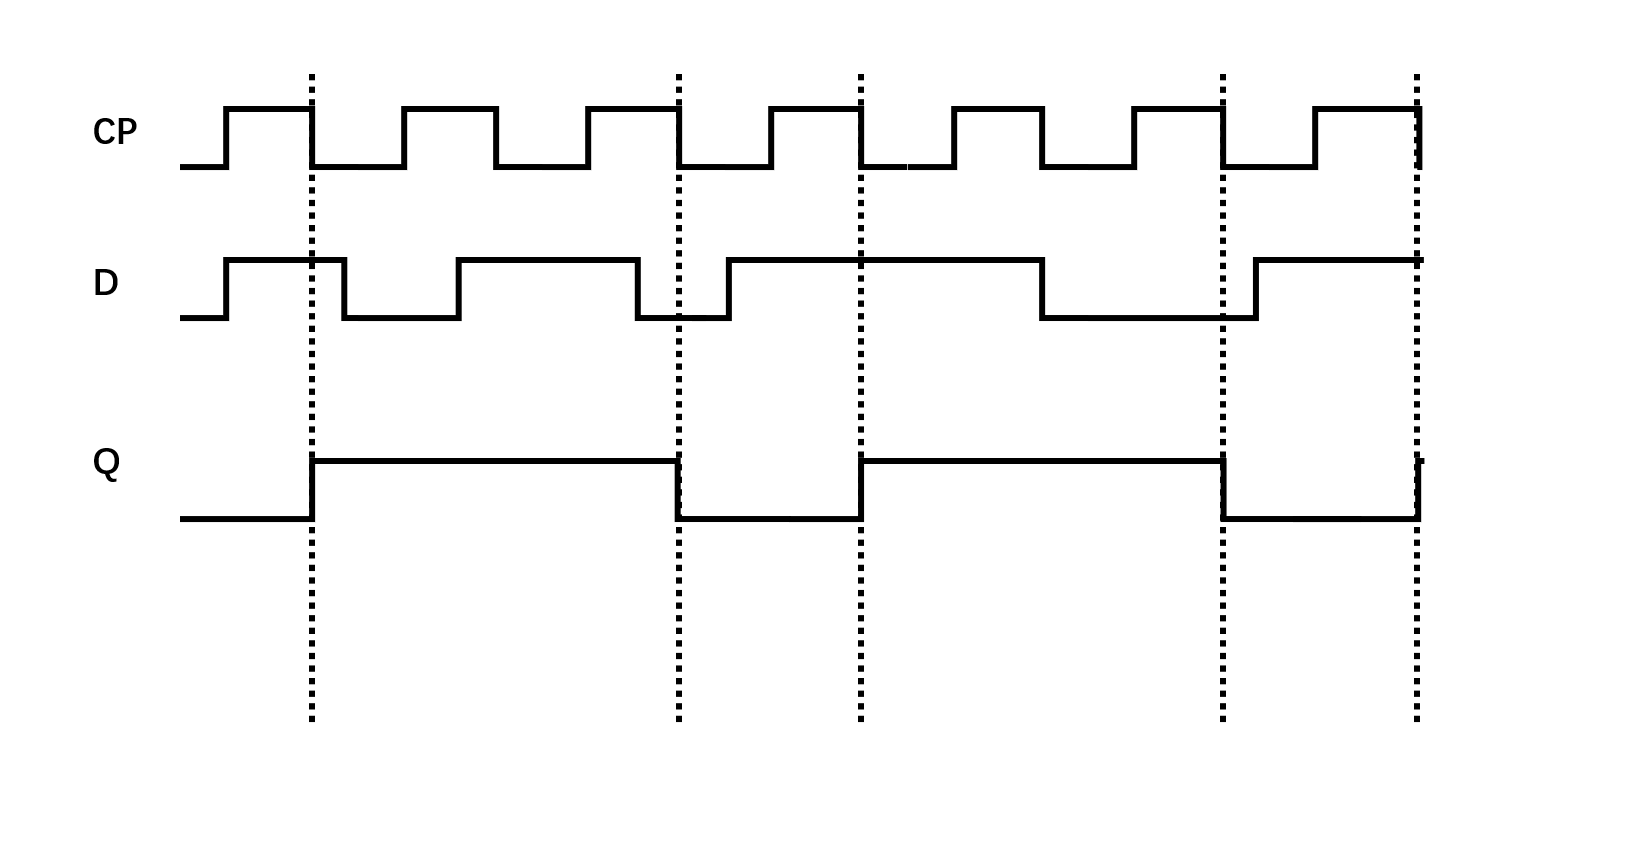
\includegraphics[width=0.6\textwidth]{image/wave_5.png}\end{center}
\end{Answer}

\begin{question}{}{}
  5-18 Draw the waveform of B and Q.
\end{question}
\begin{Answer}
同理可得其状态转移方程，根据题目所述，绘制如图：
\begin{center}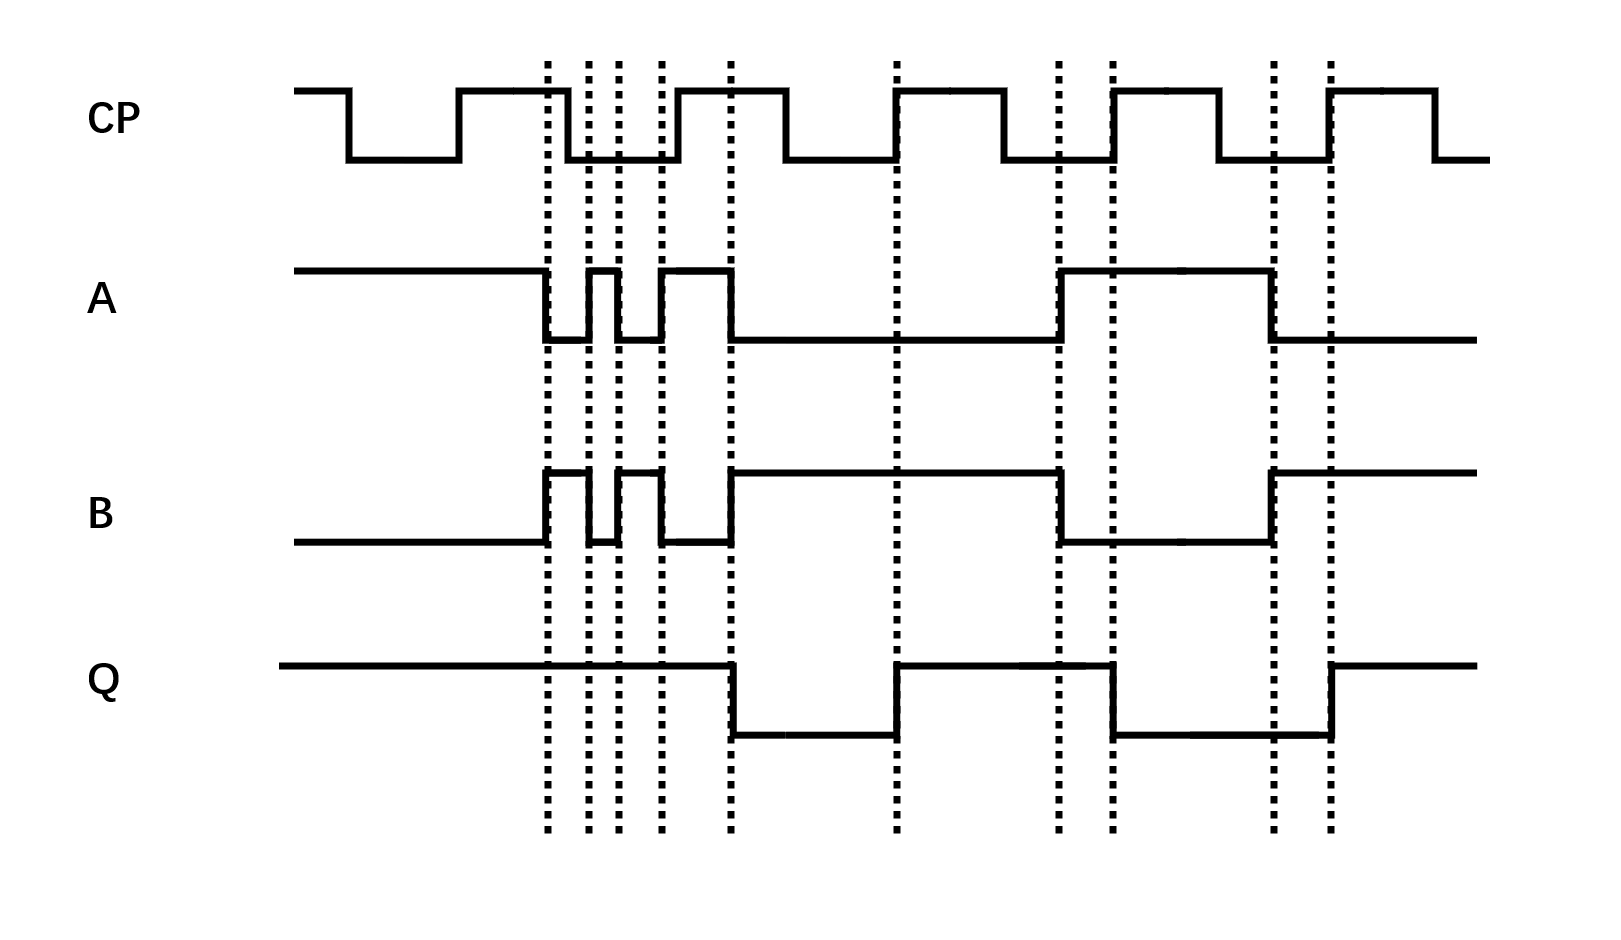
\includegraphics[width=0.6\textwidth]{image/wave_6.png}\end{center}
\end{Answer}

\begin{question}{}{}
  5-21 Draw the waveform and find the mistake of the code.
\end{question}
\begin{Answer}
问题在于，当$J=1$和$K=1$时：
假设CP为1：

$$WRn=~(1\&1\&WQ)=~WQ$$
$$WSn=~(WQn\&1\&1)=~WQn$$

反馈回路的竞争可能会导致WQ和WQn之间不断地翻转，这会使仿真工具进入无穷循环，导致VCD文件卡住。

解决方案：
在某些情况下，通过添加延迟或状态检测，可以避免竞争状态或震荡。
可以修改测试平台，以便在特定状态下暂停或确保在切换之前有足够的时间进行稳定，
或者修改模块，在 J=1 和 K=1 的情况下，增加适当的逻辑以防止输出的不稳定。
或者，使用寄存器来存储并输出稳定状态，根据实际需求调整逻辑处理，以确保模块能够正常工作。

忽略$J=1$和$K=1$时的波形图如下：

\begin{center}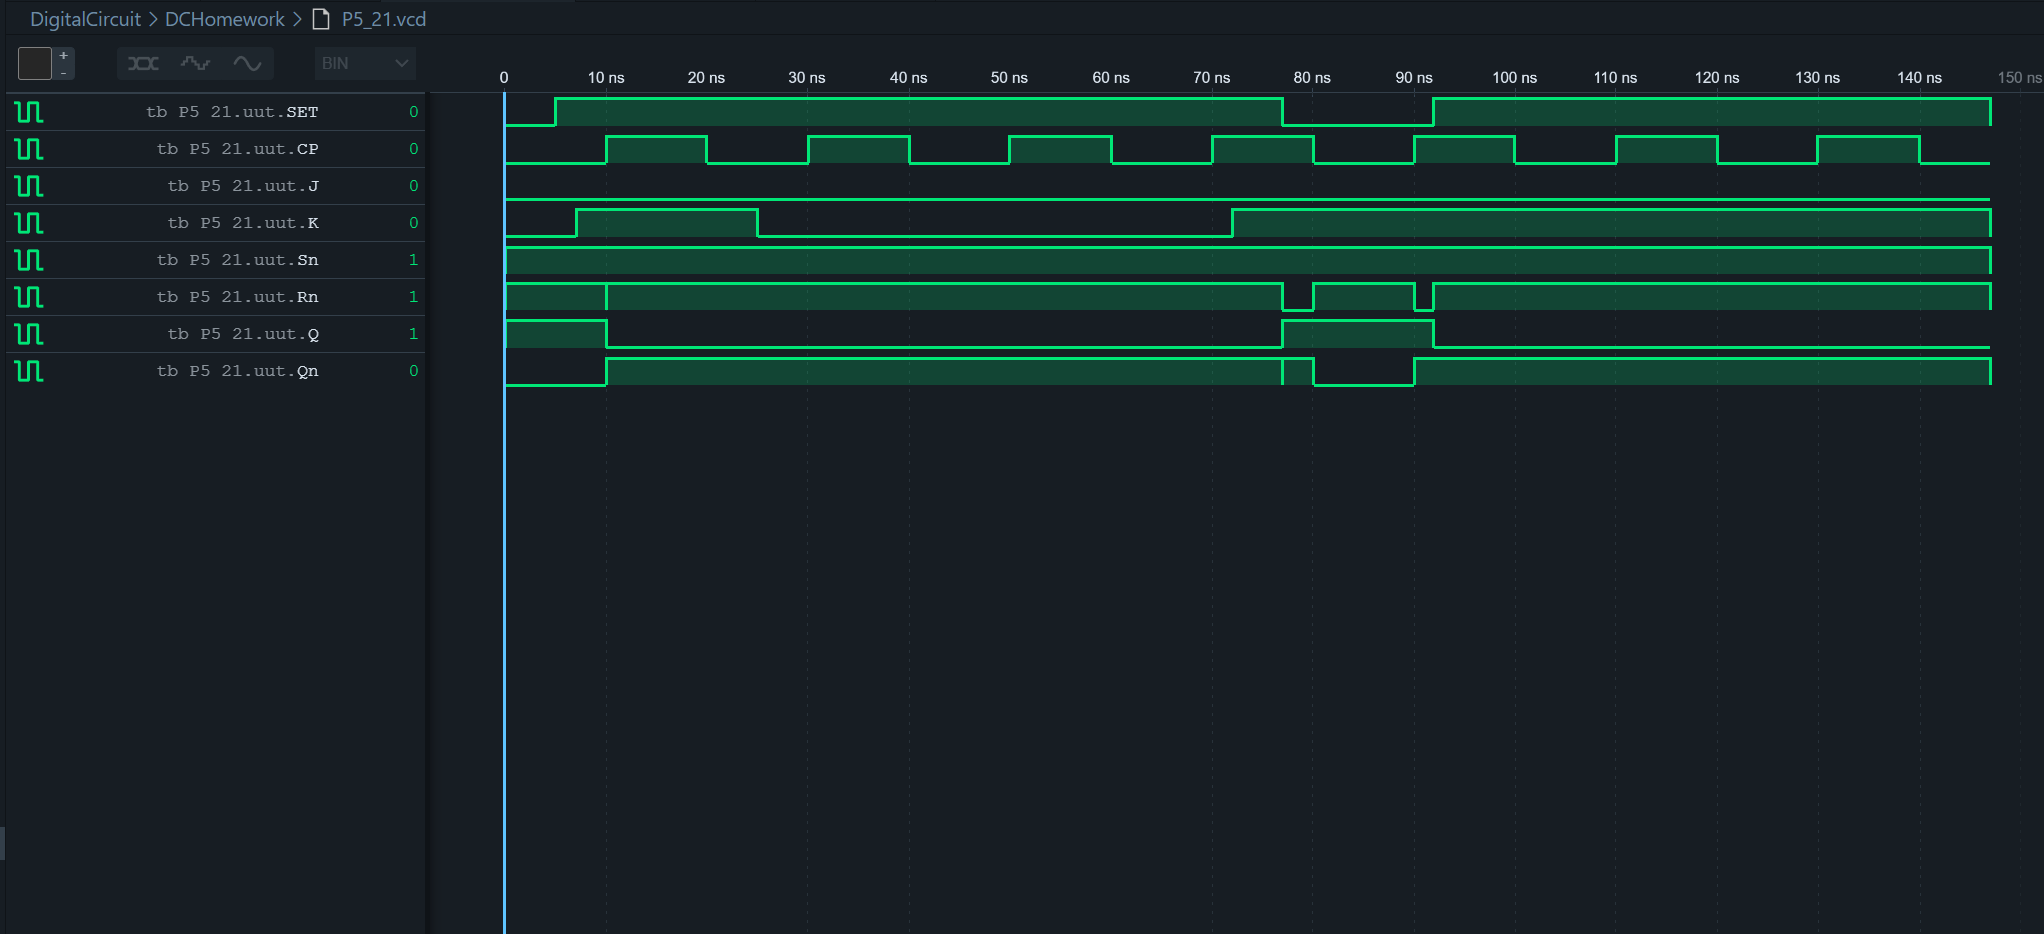
\includegraphics[width=1\textwidth]{image/wave_7.png}\end{center}

\end{Answer}

\begin{question}{}{}
  5-22 Draw logic diagram and waveform of the module.
\end{question}
\begin{Answer}
由题目易得，逻辑图如下：

\begin{center}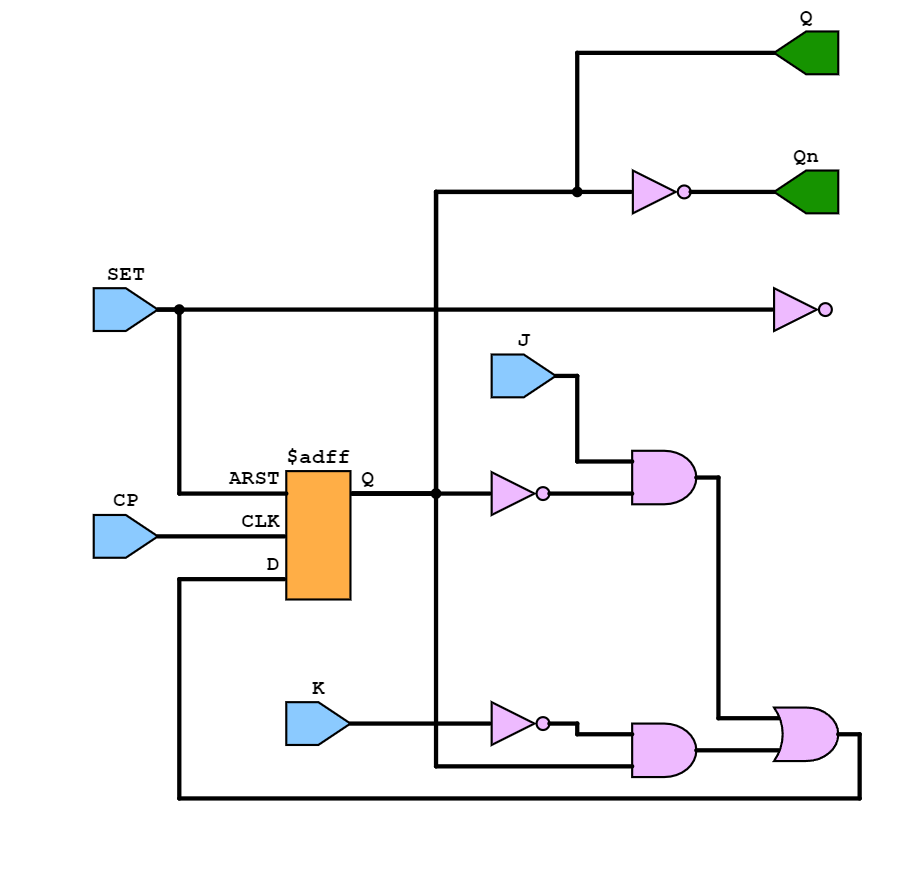
\includegraphics[width=0.6\textwidth]{image/wave_8.png}\end{center}

波形图如下：
\begin{center}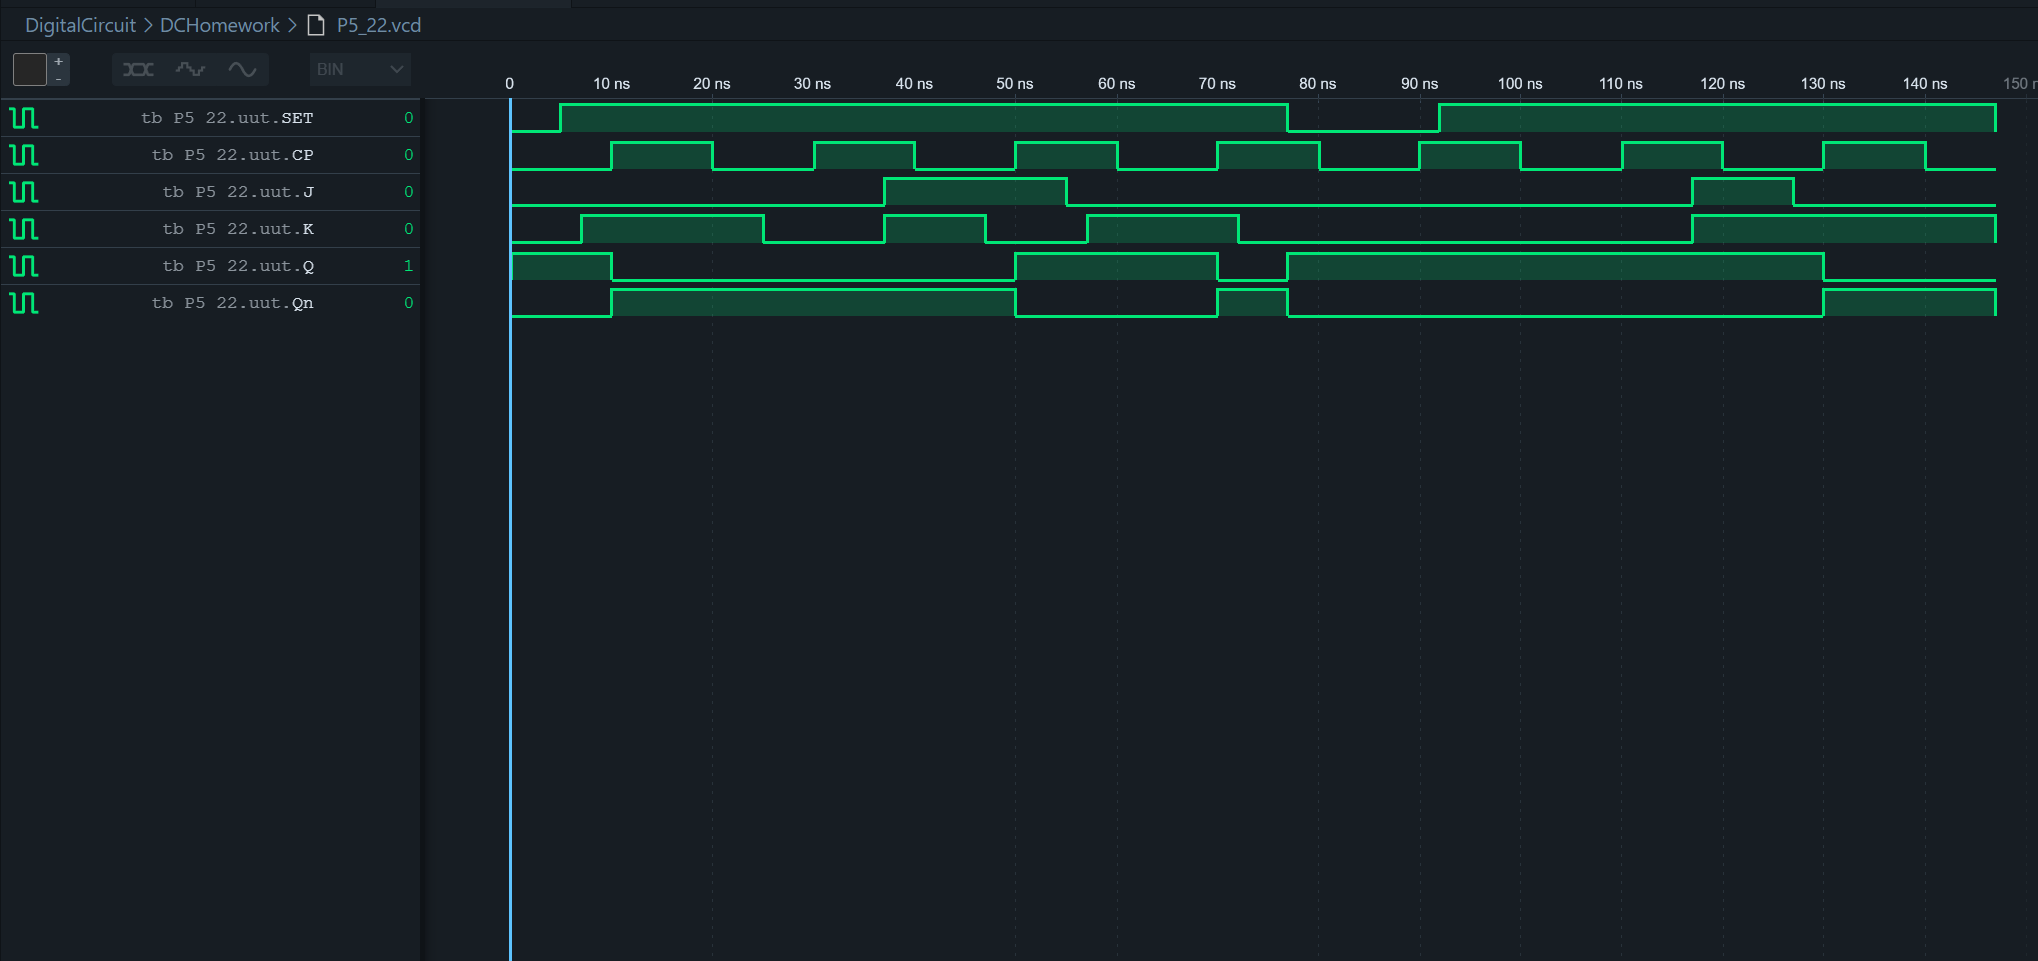
\includegraphics[width=1\textwidth]{image/wave_9.png}\end{center}
\end{Answer}
\begin{flushright}\begin{tabular}{rl}
  姓名: & 李俊洁\\
  班级: & 计算机2204 \\
  学号: & 20225443 \\
  课程: & 数字逻辑与数字系统 \\
  日期: & May 25, 2024 \\
  制作: & \LaTeX \\
  & 感谢您的批阅！
\end{tabular}\end{flushright}
\end{document}